\section{Is that all?}
Further, YARP contains simple libraries for managing images and other sensory data types, including the possibility of trasmitting them through the network. For example, images can be grabbed on one node and sent, in parallel, by using the IP-multicast protocol to many nodes for parallel processing. With certain limitations, this is efficient enough to parallelize image processing which is typically time consuming on current processors.

YARP also comes with libraries for shielding the dependencies on the robot hardware. Clearly such a mechanism could never be fail-proof given the number and combinations of different control cards, robot structure, etc. We attempted at shielding these dependencies so that future hardware replacement is possible with a minimal amount of work. This encapsulation comes into two different libraries: {\bf libYARP\_dev} and {\bf libYARP\_robot}. The first library deals with the encapsulation and standardization of different hardware cards, the latter with the robot architecture itself.

The following sections describe first how to compile the existing libraries and then how to prepare new device drivers to be included in the generic YARP structure, finally, we will delve deep into the preparation of a new robot architecture.
 
\section{Preparing libYARP\_math}
The mathematical library of YARP is a fairly simple and straightforward set of classes mostly used to support a generic vector and matrix type. As typical of YARP, the appropriate type definitions for sending and receiving vectors and matrices are provided. This allows sending vectors and matrices of double precision numbers through the network, exactly as for the other YARP types. Ideally, we would like to avoid implementing a full-fledged math library that would be outside the scope of YARP itself and rather provide the minimal amount of support leaving to the user the task of interfacing to their preferred packages. This, we believe, is in agreement with the general design philosophy of YARP: be respectful of the user's preferences. An interface to the GNU scientific library would be perhaps most welcome.

The math library can be compiled both by means of the VisualStudio project (on Windows), makefile on Linux, QNX, and MacOS. As for the other libraries you have the choice of using the perl scripts to configure and compile it (recommended) or opening the project yourself, compile, and then copy the libraries and headers to the appropriate locations. Both procedures are sketched next.

\subsection{Perl scripts}
Using perl is fairly trivial in this case. Just run the {\em configure.pl} script (e.g. by typing perl configure.pl). The following output (or a similar one) should be printed on your terminal windows:

\begin{verbatim}
Entering configure process of YARP math support library...
'uname' is not recognized as an internal or external command,
operable program or batch file.
Ready to start...
Now I'm going to ask a few questions to help building the configuration. 
For pathnames you can use (type) the pre-defined value $YARP_ROOT that 
I've verified as: "D:\Users\pasa\Repository\yarp"

Please, use always the forward slash as a separator!
I determined already that you're running on a supported OS: winnt
Would you like to set a default for library compilation?
Clean first: i.e. rebuild libraries? [TRUE]
\end{verbatim}

This procedure is completely equivalent to the libYARP\_OS library compilation. All what you have to do is to decide if your need a rebuild (clean first), whether you would like to compile debug and/or optimized and to install after compilation. For example:

\begin{verbatim}
Debug mode? [TRUE]
Release mode (optimization on)? [TRUE]
Install after compile? [TRUE]
We're done for now, the context file is being updated: 
"D:\Users\pasa\Repository\yarp/conf/context.conf"
Done!
\end{verbatim}

This creates the appropriate configuration options in the \$YARP\_ROOT/conf/context.txt file which are then used by {\em build.pl}. To compile, run the {\em build.pl} script. The output should look like this one:

\begin{verbatim}
Entering compile process of YARP math library...
'uname' is not recognized as an internal or external command,
operable program or batch file.
Ready to start...
Working with: D:\Users\pasa\Repository\yarp/conf/context.conf

Cleaning...
Deleting intermediate files and output files for project 
'libYARP_math - Win32 Debug'.
Deleting intermediate files and output files for project 
'libYARP_math - Win32 Release'.


Compiling debug
------Configuration: libYARP_math - Win32 Debug--------------
Compiling...
YARPLU.cpp
YARPMatrix.cpp
YARPRobotMath.cpp
YARPSVD.cpp
Generating Code...
Creating library...

libYARP_mathd.lib - 0 error(s), 0 warning(s)
\end{verbatim}

\noindent and the procedure will complete, in this case, with full installation.


\subsection{Do it yourself}
Even if you decided not to use the perl scripts compilation is pretty simple. In Windows you need to open the libYARP\_math.dsw from VisualStudio, choose the configuration (Debug or Release) and start the compiler. When it is done, you have to manually copy headers and libraries:
\begin{itemize}
\item copy all .lib files from ./lib/winnt into \$YARP\_ROOT/lib/winnt
\item copy all .h files from ./include/yarp into \$YARP\_ROOT/include/yarp
\end{itemize}

In Linux, the Makefile provided takes care of compiling everything. As a last step copy the libraries by typing:
\begin{quote}
{\tt cp ./lib/linux/*.a \$YARP\_ROOT/lib/linux}
\end{quote}

\noindent and the headers as shown earlier. 



\section{Signal Processing}
The YARP signal processing library (libYARP\_sig) has several basic types for dealing with images and sending them from one machine to another for parallel processing. As for the libYARP\_math library, the signal processing library does not contain an elaborated set of visual processing primitives but rather relies on the user to provide implementations. YARP signal processing classes mostly deal with the communication of data across the network. Some basic primitives are provided and, for images, integration with the {\em open cv} data types.

The basic data type used in libYARP\_sig is the {\em YARPGenericImage}. This is a container class managing an array of pixels of an unspecified type and size. In practice the internal pixel array is always a chunk of memory. The actual type exported to user code is a class template declared as follows:

\begin{verbatim}
  template <class T>
    class YARPImageOf : public YARPGenericImage
\end{verbatim}

\noindent which allows arbitrary data types T to be used as pixel types. The library provides already the most commonly used pixel types such as RGB, HSV, Mono, etc. Images can be easily transmitted across the network using YARP ports. The appropriate port would be declared as:

\begin{verbatim}
  YARPInputPortOf<YARPGenericImage> input_port;
\end{verbatim}

\noindent that is, of type YARPGenericImage. At run-time the port would know the actual pixel type and refer the an image to the actual data type. For efficiency, images can also refer (i.e. point to) data or other images allocated in advance. In practice, a copy is seldom required, and often the processing can happen in place. For example, considering the port declaration above:

\begin{verbatim}
  YARPImageOf<YarpPixelMono> in;
  .
  .
  .
  in.Refer (input_port.Content());	
\end{verbatim}

Similarly, the signal processing library has classes for sound data transfer: {\em YARPSoundBuffer}. The sound buffer is a generic 8-bit array that can be trasmitted through ports (as for images). The sound buffer is much simpler in structure than images and thus it is the preferred method for handling raw data. The procedure to compile the libYARP\_img is very similar to the math library and it is reported below only for completness. Do not bother in actually reading it.

\subsection{Perl scripts}
Using perl is fairly trivial in this case: just run the {\em configure.pl} script (e.g. by typing perl configure.pl). The following output (or a similar one) should be printed on your terminal windows:

\begin{verbatim}
Entering configure process of YARP signal processing library...
'uname' is not recognized as an internal or external command,
operable program or batch file.
Ready to start...
Now I'm going to ask a few questions to help building the configuration. 
For pathnames you can use (type) the pre-defined value $YARP_ROOT that 
I've verified as: "D:\Users\pasa\Repository\yarp"

Please, use always the forward slash as a separator!
I determined already that you're running on a supported OS: winnt
Do you want to include IPL support (emulation otherwise)? [NO]
\end{verbatim}

This procedure is completely equivalent to the libYARP\_OS and libYARP\_math library compilation. The IPL support flag is not actually used for the time being; any value will do. All what you have to do is to decide if your need a rebuild (clean first), whether you would like to compile debug and/or optimized and to install after compilation. For example:

\begin{verbatim}
Would you like to set a default for library compilation?
Clean first: i.e. rebuild libraries? [TRUE]
Debug mode? [TRUE]
Release mode (optimization on)? [TRUE]
Install after compile? [TRUE]
We're done for now, the context file is being updated: 
"D:\Users\pasa\Repository\yarp/conf/context.conf"
Done!
\end{verbatim}

This creates the appropriate configuration options in the \$YARP\_ROOT/conf/context.txt file which are then used by {\em build.pl}. To compile, run the {\em build.pl} script. The output should look like this one:

\begin{verbatim}
Entering compile process of YARP signal processing libraries...
'uname' is not recognized as an internal or external command,
operable program or batch file.
Ready to start...

Cleaning...
Deleting intermediate files and output files for project 'libYARP_sig 
- Win32 Debug'.
Deleting intermediate files and output files for project 'libYARP_sig 
- Win32 Release'.


Compiling debug
----------Configuration: libYARP_sig - Win32 Debug-----------------

Compiling...
cvbase.cpp
YARPImage.cpp
YARPImageFile.cpp
YARPImageUtils.cpp
YARPSimpleOperations.cpp
Generating Code...
Creating library...

libYARP_sigd.lib - 0 error(s), 0 warning(s)

\end{verbatim}

\noindent and the procedure will complete, in this case, with full installation.


\subsection{Do it yourself}
Even if you decided not to use the perl scripts compilation is pretty simple. In Windows you need to open the libYARP\_img.dsw from VisualStudio, choose the configuration (Debug or Release) and start the compiler. When it is done, you have to manually copy headers and libraries:
\begin{itemize}
\item copy all .lib files from ./lib/winnt into \$YARP\_ROOT/lib/winnt
\item copy all .h files from ./include/yarp into \$YARP\_ROOT/include/yarp
\end{itemize}

In Linux, the Makefile provided takes care of compiling everything. As a last step copy the libraries by typing:
\begin{quote}
{\tt cp ./lib/linux/*.a \$YARP\_ROOT/lib/linux}
\end{quote}

\noindent and the headers as shown earlier. 


\subsection{OpenCV support}
The image classes are internally already compatible with the {\em open cv} data structure (and IPL). To enable this feature you need to define the preprocessor symbol {\em HAVE\_IPL} and for instance set it equal to 1. You need to add also the IPL or the {\em open cv} include files as for example:

\begin{verbatim}
  #include <ipl/ipl.h>
\end{verbatim}

A cast operator allows calling any IPL function using YARPImage's as arguments.
 
  
\section{Preparing libYARP\_dev}
The device driver library is a heterogeneous collection of various modules. It is composed of a few files of general use (mostly class templates) and a set of device drivers developed for the robot mentioned in the introduction (see section \ref{sect:numbers}). For each device driver we are providing only the appropriate header files and libraries for linking the code correctly while the actual device driver needs to be acquired through the specific hardware manifacturer.

The directory tree thus contains the usual {\em src} and {\em include} subdirectories and then one directory per device driver. This is further subdivided according to the following example (taken from the {\em picolo} device driver, a BT848-based frame grabber):

\begin{table}[h]
	\centering
		\begin{tabular}{|c|c|c|}
		\hline
			1st level & 2nd level & 3rd level \\
			\hline \hline
			winnt & dd\_orig & bin \\
			 &  & include \\
			 &  & lib \\
			 & yarp & \\
			\hline
			linux & dd\_orig & include \\
			 &  & lib \\
			 &  & src \\
			 & yarp & \\
			\hline
		\end{tabular}
\end{table}

The {\em dd\_orig} subtree contains all what is needed to write code and link to the actual driver libraries (typically provided by the hardware manufacturer). Sometimes there is a library, in other cases, the source code is available (not frequently). The YARP device files are contained under {\em yarp} and they are compiled and headers copied to the appropriate location (e.g. \$YARP\_ROOT/include/yarp) during installation. As we will see, once compiled and linked the {\em dd\_orig} files are no longer needed and do not require to be installed anywhere in the system. This is convenient for preparing pre-compiled distributions for certain architectures.

Compilation for existing configurations can be done through the usual pair of perl scripts. Upon running {\em configure.pl}, the following text should show up on your terminal window:

\begin{verbatim}
Entering configure process of YARP device drivers...
'uname' is not recognized as an internal or external command,
operable program or batch file.
Ready to start...
Now I'm going to ask a few questions that I need for configuring the device 
drivers.
For pathnames you can use (type) the pre-defined value $YARP_ROOT that I've 
verified as: "D:\Users\pasa\Repository\yarp"

Please, use always the forward slash as a separator!
I determined already that you're running on a supported OS: winnt
I also imagine you've compiled YARP_OS, I'm not checking for it so please 
make sure you've run "configure.pl" and "build.pl" for YARP_OS.

You are going to provide information on your hardware configuration here. 
If this procedure isn't clear to you, please, have a look at the 
documentation
To start, provide a name for your hardware context. This will be merged 
with the OS name to provide our installation means of distinguishing this 
specific hardware

What is your hardware name? [babybot]
\end{verbatim}

After the usual startup checks, the script confirms the definition of the \$YARP\_ROOT environment variable and then asks for the hardware name. This is a symbolic name (a string) that identifies the platform (the robot) you are about to compile for. Valid names are for example contained in \$YARP\_ROOT/conf/ (apart from {\em install}). You type one of the names available or confirmed the proposed name by pressing {\em return}. To continue this example, let's imagine we are content with the babybot configuration. This is not too important for compiling the device drivers but rather it is required later to compile the libYARP\_robot.

The next step is to provide the usual compilation options as for libYARP\_OS. We have already seen a similar procedure earlier.

\begin{verbatim}
Then your context specific directories are going to be called: "babybot"
These are the standard flags for compiling the library
Clean first: i.e. rebuild libraries? [FALSE]
Compile debug version? [TRUE]
Compile release (optimized)? [TRUE]
Install after build? [TRUE]
Browsing through the list of available device drivers
In case you don't know what to do, it's no harm including all available 
drivers
Would you like to add "androidworld" to the project [YES]?
\end{verbatim}

The scripts goes through all the available device drivers and asks which are to be included in the device library. Only those which are selected are actually included into the library. The scripts creates a new VisualStudio project on Windows and a Makefile on Linux. An example of this procedure (for the {\em babybot} project) is shown below:

\begin{verbatim}
Would you like to add "androidworld" to the project [YES]?
Would you like to add "cyberglove" to the project [YES]? n
Would you like to add "dragonfly" to the project [YES]? n
Would you like to add "esdcan" to the project [YES]? n
Would you like to add "fob" to the project [YES]? n
Would you like to add "galil" to the project [YES]? y
Would you like to add "joypres" to the project [YES]? n
Would you like to add "jr3" to the project [YES]? y
Would you like to add "mei" to the project [YES]? y
Would you like to add "nidaq" to the project [YES]? y
Would you like to add "null" to the project [YES]? n
Would you like to add "null_grabber" to the project [YES]? n
Would you like to add "picolo" to the project [YES]? y
Would you like to add "sound" to the project [YES]? y
Would you like to add "valuecan" to the project [YES]? n
We're done for now, the context file has been updated: 
"D:\Users\pasa\Repository\yarp/conf/context.conf"
A new project reflecting your choices has been created in "./src"
Type "build.pl" later to start the build process

Now I need to create a few additional include files
I might need to ask you more questions...

Good! It seems you have the right directories for the hardware context 
you've just chosen
Generating "YARPConfigRobot.h"
Copying D:\Users\pasa\Repository\yarp/conf/babybot/YARPConfig_babybot.h.
You've got also a "vocab" file for YARPBottles, I'm including it.
Done!
\end{verbatim}

The scripts checks also that the {\em babybot} context files are present (see section \ref{} for the creation of a new platform) and prepares the appropriate {\em YARPRobotConfig.h} file. Finally, it sees there is a valid {\em YARPVocab} file containing definitions of the message IDs available for {\em YARPBottle}s and thus includes it.

Now, we are ready to compile the libYARP\_dev library. Just run {\em build.pl}, you should see something similar to the following output:

\begin{verbatim}
Entering compile process of YARP_dev libraries...
'uname' is not recognized as an internal or external command,
operable program or batch file.
Ready to start...
Working with: D:\Users\pasa\Repository\yarp/conf/context.conf

Cleaning...
Deleting intermediate files and output files for project 
'libYARP_dev_babybot - Win32 Debug'.
Deleting intermediate files and output files for project 
'libYARP_dev_babybot - Win32 Release'.


Compiling debug
--------------------Configuration: libYARP_dev_babybot - 
Win32 Debug--------------------
Compiling...
YARPControlBoardUtils.cpp
YARPAndroidDeviceDriver.cpp
YARPGalilDeviceDriver.cpp
YARPJR3DeviceDriver.cpp
YARPMEIDeviceDriver.cpp
YARPNIDAQDeviceDriver.cpp
\end{verbatim}

\noindent and so on. As a last step, the build procedure creates a single library by concatenating the existing device driver libraries. It scans the {\em dd\_orig} subdirectories, reads the library files and merges them into a single file.

\begin{verbatim}
Now building libraries...
Compacting libraries: ".\galil\winnt\dd_orig\lib\DMC32.lib" ".\galil\winnt
\dd_orig\lib\DMCMLIB.lib" ".\jr3\winnt\dd_orig\lib\jr3pci_lib.lib" ".\mei\
winnt\dd_orig\lib\medvc60f.lib" ".\nidaq\winnt\dd_orig\lib\nidaq32.lib" ".
\nidaq\winnt\dd_orig\lib\nidex32.lib" ".\picolo\winnt\dd_orig\lib\Picolo32
.lib"
Microsoft (R) Library Manager Version 6.00.8447
Copyright (C) Microsoft Corp 1992-1998. All rights reserved.

DMCMLIB.lib(DMCMLIB.dll) : warning LNK4006: __NULL_IMPORT_DESCRIPTOR alrea
dy defined in DMC32.lib(DMC32.dll); second definition ignored
medvc60f.lib(medvc60f.dll) : warning LNK4006: __NULL_IMPORT_DESCRIPTOR alr
eady defined in DMC32.lib(DMC32.dll); second definition ignored
nidaq32.lib(nidaq32.dll) : warning LNK4006: __NULL_IMPORT_DESCRIPTOR alrea
dy defined in DMC32.lib(DMC32.dll); second definition ignored
nidex32.lib(NIDEX32.dll) : warning LNK4006: __NULL_IMPORT_DESCRIPTOR alrea
dy defined in DMC32.lib(DMC32.dll); second definition ignored
Picolo32.lib(Picolo32.dll) : warning LNK4006: __NULL_IMPORT_DESCRIPTOR alr
eady defined in DMC32.lib(DMC32.dll); second definition ignored
Microsoft (R) Library Manager Version 6.00.8447
Copyright (C) Microsoft Corp 1992-1998. All rights reserved.
\end{verbatim}

Duplicate symbols warnings are typically of no concern under Windows.



\section{YARPDeviceDriver}
We start by introducing the YARP device driver templates and wrappers through an example. We consider the already mentioned BT848 frame grabber. This is a fairly simple device with only a few functions but enough to illustrate the principles. A more complex set of classes is shown later.

The first component of the hierarchy is the YARPDeviceDriver template class. This is meant to be the base class of all device driver abstractions (within YARP of course). Check the {\em YARPDeviceDriver.h} file for details. The declaration of the template is the following:

\begin{verbatim}
template <class SYNC, class DERIVED> 
    class YARPDeviceDriver
\end{verbatim}

\noindent where SYNC is the synchronization object to use by the class and DERIVED is the type derived from the device driver. The SYNC object must support the {\em Post} and {\em Wait} methods. Valid examples are the {\em YARPNullSemaphore} and {\em YARPSemaphore} provided in the libYARP\_OS library. We should declare our frame grabber device driver as:

\begin{verbatim}
class YARPPicoloDeviceDriver : 
    public YARPDeviceDriver<YARPNullSemaphore, YARPPicoloDeviceDriver>, 
    public YARPThread
\end{verbatim}

\noindent this is called {\em YARPPicoloDeviceDriver} after the name of the card we actually used on one of our robots. As shown here, the device driver derives from the YARP template and also from the {\em YARPThread} class since it internally manages concurrent access to the acquisition buffers. In this case, since mutual exclusion is not required, the SYNC object is a {\em YARPNullSemaphore}.

The {\em YARPDeviceDriver} supports three methods only: {\em open}, {\em close}, and {\em IOCtl}. The device driver can be only opened, closed or controlled. The three methods are declared as follows:
\begin{itemize}

\item open.
\begin{verbatim}
      virtual int open(void *) = 0;		
\end{verbatim}
where the {\em void *} argument is used to pass a generic type (e.g. a struct) containing the initialization paramters.

\item close.
\begin{verbatim}
      virtual int close() = 0;
\end{verbatim}
which closes the device driver.

\item IOCtl.
\begin{verbatim}
      int IOCtl(int cmd, void *data);
\end{verbatim}
The commands to the actual hardware are sent though this methods, the {\em cmd} argument is the message number (or ID) and {\em data} is the additional data/params required for the actual execution of the function.

\end{itemize}

The goal of the implementation of the device driver in YARP is then that of shielding completely any call to the original libraries through this class (the {\em YARPPicoloDeviceDriver}). With the same spirit, the original device header files are not included from the YARP driver header file so that, once compiled, YARP no longer requires anything from the original manufacturer library. To help shielding the implementation any type required by the driver is allocated through a {\em void *} variable called {\em system\_resources}. Typically this is a pointer to a class allocated during the device initialization containing all the device variables. In our example, the {\em YARPPicoloDeviceDriver} looks liek this:

\begin{verbatim}
    class YARPPicoloDeviceDriver : 
      public YARPDeviceDriver<YARPNullSemaphore, YARPPicoloDeviceDriver>, 
      public YARPThread
    {
    private:
      YARPPicoloDeviceDriver(const YARPPicoloDeviceDriver&);
      void operator=(const YARPPicoloDeviceDriver&);

    public:
      YARPPicoloDeviceDriver();
      virtual ~YARPPicoloDeviceDriver();

      virtual int open(void *d);
      virtual int close(void);

      virtual int acquireBuffer(void *);
      virtual int releaseBuffer(void *);
      virtual int waitOnNewFrame (void *cmd);
      virtual int getWidth(void *cmd);
      virtual int getHeight(void *cmd);

    protected:
      void *system_resources;

      virtual void Body(void);
    };
\end{verbatim}

For the moment, it is important to note the private copy contructor and copy operator (this is done to avoid the user blissfully creating copies of the device driver) and the {\em system\_resources} variable as mentioned above. We then overload the {\em open} and {\em close} methods. Also, note that the {\em open} method accept a parameter through a {\em void *}. This contains a set of parameters, typically contained in a struct, that defines the initialization of the device. For example: 

\begin{verbatim}
    struct PicoloOpenParameters
    { 
      ...
      int _video_type;
      int _size_x;
      int _size_y;
    }
\end{verbatim}

\noindent with the obvious meaning of the parameters. As we said, the device driver methods are invoked only through the {\em IOCtl}. This is obtained by calling {\em IOCtl} with a message number as first argument. The message number indexes  a table of function pointers which then invoke the appropriate method. Consequently, we are required to define the type of messages accepted by all frame grabber type device drivers which in practice become the standard interface to the physical device. The main abstraction is a message system! In our example, we create a {\em YARPFrameGrabberUtils.h} file with a list of messages:

\begin{verbatim}
    enum FrameGrabberCmd
    {
      FCMDAcquireBuffer = 1,
      FCMDReleaseBuffer = 2,
      FCMDWaitNewFrame = 3,
      FCMDGetSizeX = 4,
      FCMDGetSizeY = 5,

      FCMDNCmds = 6
    };
\end{verbatim}

This represents all that can be done with the device driver: the actual interface between the harware and our software layer. Note that this is a separate file because many devices might share the same messages (many different frame grabbers are subsumed under the same interface). For the actual implementation, the frame grabber example, as mentioned earlier, defines a class embedding some of the details of the specific library (see next):

\begin{verbatim}
    class PicoloResources
    {
    public:
      PicoloResources (void) : _bmutex(1), _new_frame(0)
      { ... }
      ~PicoloResources () { _uninitialize (); }

      enum { _num_buffers = 3 };

      PICOLOHANDLE _picoloHandle;	

      ...
    };
\end{verbatim}

\noindent where the type {\em PICOLOHANDLE} is specific to the original device library. Clearly, you are very free here to create the resource class that suits your needs. The implementation must be hidden to the interface, thus the resource class should be defined and used only within the implementation of the device driver. For instance, the type {\em PICOLOHANDLE} should never appear in the interface. The device driver constructor should then allocate the {\em system\_resources} class and create the function pointers table as shown next:

\begin{verbatim}
    YARPPicoloDeviceDriver::YARPPicoloDeviceDriver(void) : 
      YARPDeviceDriver<YARPNullSemaphore, YARPPicoloDeviceDriver>(FCMDNCmds)
    {
      system_resources = (void *) new PicoloResources;
      ACE_ASSERT (system_resources != NULL);

      // for the IOCtl call.
      m_cmds[FCMDAcquireBuffer] = &YARPPicoloDeviceDriver::acquireBuffer;
      m_cmds[FCMDReleaseBuffer] = &YARPPicoloDeviceDriver::releaseBuffer;
      m_cmds[FCMDWaitNewFrame] = &YARPPicoloDeviceDriver::waitOnNewFrame;
      m_cmds[FCMDGetSizeX] = &YARPPicoloDeviceDriver::getWidth;
      m_cmds[FCMDGetSizeY] = &YARPPicoloDeviceDriver::getHeight;
    }
\end{verbatim}

Note that we are providing the size of the table of function pointers to the {\em YARPDeviceDriver} constructor that is taking care of allocating it. A default empty implementation of all messages is provided by the base class which makes safe to call the driver for messages that it does not implement. A destructor should be implemented, obviously taking care of freeing the memory allocated in the costructor. The message methods (those in the list above) are of type:

\begin{verbatim}
      typedef int (DERIVED::*cmd_function_t)(void *); 
\end{verbatim}

\noindent where {\em DERIVED} is the class derived from the {\em YARPDeviceDriver}. As a last step in the preparation of the device driver the {\em open} and {\em close} methods must be implemented. They must respectively initialize and uninitialize the device driver and, in this case, unlike the costructor and destructor, start the communication with the physical layer. The {\em open} method accept a parameter (a {\em void *}) that can be used to configure the device driver. You can check the declarations in {\em YARPDeviceDriver.h}.

An example of the implementation of a method that reads something from the {\em system\_resources} variable is shown below:

\begin{verbatim}
    int YARPPicoloDeviceDriver::getWidth (void *cmd)
    {
      *(int *)cmd = RES(system_resources)._nWidth;
      return YARP_OK;
    }
\end{verbatim}

\noindent where {\em RES} is only a cast to the appropriate type for accessing the {\em system\_resources}.

\begin{figure}[tb]
\centerline{
%\psfig{figure=fig-port-portlets.eps}
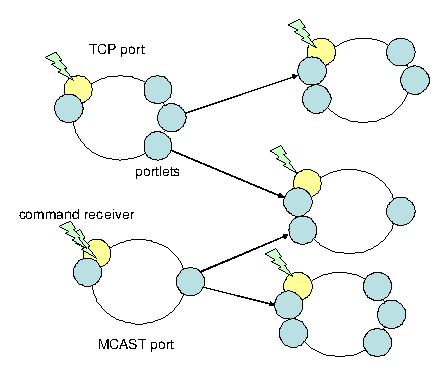
\includegraphics[width=7cm]{fig-port-portlets}
}
\caption[Interprocess communication model]{ 
%
This is supposed to be the class hierarchy diagram.
%
}
\label{fig:yarp-port}
\end{figure}



\section{The libYARP\_robot}
The next step of the YARP abstraction is carried out through the robot library: libYARP\_robot. The goal of this library is that of providing a standard interface and easy hardware replacement at the cost of some added complexity of the overall coding structure. The rationale beyond the robot libray is that of allowing diverse robotic components such as heads and arms and various different control cards to be used by a common software component. This consists of three elements:

\begin{itemize}
\item {\bf robot component}: e.g. the robot head or the visual sensors control
\item {\bf hardware interface card}: e.g. the motor control card or the frame grabber
\item {\bf details of the interface}: e.g. how the motor control card is connected to the robot head
\end{itemize}

These three elements are represented by three classes that are combined to build a control element such as that controlling the robot head. The robot component is described through a derivation from a template C++ class specific to the type of object being controlled (e.g. a control card rather than a frame grabber). This is customized by specializing the template class. The template is typically a function of two parameters called the {\em ADAPTER} and the {\em PARAMETERS}. The {\em ADAPTER} is derived from a {\em YARPDeviceDriver}; the {\em PARAMETERS} class is not derived from a base class but it rather specific to the type of device. The parameters are gathered here, that is, all differences from two different use of the same control card (for the a similar application though) are concentrated here. Lately, certain devices have a parameter class derived from a common base in a tentative to rationalize the creation of new components. 

Considering again the example we presented for the libYARP\_dev, the generic component for the frame grabber is defined as:

\begin{verbatim}
    template <class ADAPTER, class PARAMETERS>
    class YARPGenericGrabber
    {
      ...
\end{verbatim}

\noindent and, in practice, the {\em YARPGenericGrabber} class contains the same methods of the adapter class (the device driver). There are two new methods with respect to the adapter class: {\em initialize} and {\em uninitialize}. The initialization is delegated to the {\em initialize} method, which can be used to solve card idiosyncrasies. Initialization code calls the adapter initialize method which can work as a placeholder for any type of initialization that might be required by specialized hardware. In short, all {\em ADAPTER}'s that are used in the {\em YARPGenericGrabber} must implement {\em initialize} and {\em uninitialize}. Note that these two methods are not in the {\em YARPPicoloDeviceDriver} since we would like to maintain the liberty of implementing different initializations for different configurations: i.e. two robots might employ the same hardware but initialize it differently.

The following example shows the interface of the {\em YARPGenericGrabber}:

\begin{verbatim}

    template <class ADAPTER, class PARAMETERS>
    class YARPGenericGrabber
    {
    protected:
      ADAPTER _adapter;		/// adapts the hw idiosyncrasies
      PARAMETERS _params;		/// actual grabber specific parameters

    public:
      YARPGenericGrabber () {}
      ~YARPGenericGrabber () {}

      int initialize (int board, int sizex, int sizey = -1);
      int uninitialize (void);
      int acquireBuffer (unsigned char **buffer);
      int releaseBuffer (void);
      int waitOnNewFrame (void);
      int getWidth (int *w);
      int getHeight (int *h);
    };
		
\end{verbatim}

The remaining methods are implemented simply by calling the {\em IOCtl} with the relative message number. As we mentioned earlier, the message types are defined in {\em YARPFrameGrabberUtils.h} for this specific example. As we have seen in the definition of the {\em YARPGenericGrabber}, it is required to derive from the device driver class to customize the adapter. This is obtained by deriving as in the following:

\begin{verbatim}
    class YARPPicoloOnBabybotAdapter : public YARPPicoloDeviceDriver
    {
      .
      .
      .
\end{verbatim}

This is basically a customization of the device driver to solve initialization idiosyncrasies. In particular, {\em initialize} and {\em uninitialize} are used to call the {\em open} and {\em close} methods of the device driver. This is convenient since our derived adapter can tweak on the parameters to do the proper initialization for the setup you are considering. The class name now refers explicitly to the experimental setup. The complete example is shown below:

\begin{verbatim}
    class YARPPicoloOnBabybotAdapter : public YARPPicoloDeviceDriver
    {
    public:
      YARPPicoloOnBabybotAdapter() : YARPPicoloDeviceDriver() {}
      virtual ~YARPPicoloOnBabybotAdapter() {}

      int initialize (YARPBabybotGrabberParams& params)
      {
        // need additional initialization? put it here.
        return open ((void *)&params);
      }

      int uninitialize (void)
      {
        // need additional termination stuff? here's the place for it.
        return close ();
      }
    };
\end{verbatim}

Finally, the parameters class must be defined. In this example, it is made to coincide with the device driver open parameters by a typedef, but any solution would do:

\begin{verbatim}
    typedef PicoloOpenParameters YARPBabybotGrabberParams;
\end{verbatim}

At this point, we still have to provide a public interface to this structure we have been creating throughout the last two sections. This is done first by following these two simple rules:
\begin{itemize}

\item constructor and destructor of the public interface call the initialize/uninitialize of the adapter respectively;

\item initialize/uninitialize of the adapter call open/close as shown above.

\end{itemize}

The result for the example of the frame grabber is shown below:

\begin{verbatim}
    template <class ADAPTER, class PARAMETERS>
    int YARPGenericGrabber<ADAPTER, PARAMETERS>
      ::initialize (int board, int sizex, int sizey /* = -1 */)
    {
      _params._unit_number = board;
      _params._video_type = 0;
      _params._size_x = sizex;
      if (sizey > 0)
        _params._size_y = sizey;
      else
        _params._size_y = sizex;

      // Calls the adapter init that parses the 
      // params appropriately.
      // This is because initialization can vary depending 
      // on the specific setup.
      return _adapter.initialize (_params);
    }
\end{verbatim}

For the generic methods instead, the {\em IOCtl} is invoked:
\begin{verbatim}
    template <class ADAPTER, class PARAMETERS>
    int YARPGenericGrabber<ADAPTER, PARAMETERS>
      ::acquireBuffer (unsigned char **buffer)
    {
      return _adapter.IOCtl (FCMDAcquireBuffer, (void *)buffer);
    }
\end{verbatim}

There is still one last step before using the newly created implementation, this is to define a new type by employing the {\em YARPGenericGrabber} template. This can be done anywhere in the code but, for convenience, we recommend creating a new header file altogether (e.g. {\em YARPBabybotGrabber.h}) containing something like the following:

\begin{verbatim}
  #include <YARPGenericGrabber.h>
  #include <YARPPicoloOnBabybotAdapter.h>

  typedef YARPGenericGrabber
   <YARPPicoloOnBabybotAdapter, YARPBabybotGrabberParams> 
   YARPBabybotGrabber;
\end{verbatim}

This completes the implementation. In the following we provide a simple checklist of what to do to prepare a new device driver.
 
 
Let:
\begin{itemize}
\item {\bf xxx} be the name of the peripheral, e.g. Picolo for a frame grabber;
\item {\bf yyy} be the name of type of the peripheral the drivers are for, e.g. FrameGrabber for a Picolo frame grabber;
\item {\bf zzz} is an architecture which uses the hardware, e.g. Babybot;
\item {\bf uuu} is the platform, e.g. winnt.
\end{itemize}

The following files are to be created:
\begin{itemize}

\item YARP{\bf xxx}DeviceDriver.h and YARPxxxDevicedriver.cpp contain the definition and the implementation of the driver (clearly distinct for every different card). The definition might contain a new type called xxxOpenParameter which is a collection of parameters required in setting up the hardware. This is an argument to the {\em open} method of the device driver class. The implementation is typically done by instantiating a class called xxxResources to hide all the harware specific resources. These files must be saved in \$YARP\_ROOT/src/libYARP\_dev/src/xxx/uuu; in the same directory a directory called ``dd\_orig'' should be created with the original device driver files (headers, libraries, etc.) needed for compiling the YARP code;

\item YARP{\bf yyy}Utils.h it can be shared with any different hardware implementing a resurce (e.g. every frame grabber). This file contains two structures: one with a list of the messages the peripheral accepts and the other one with the data type it uses. Yarp{\bf yyy}Utils.h resides in \$YARP\_ROOT/src/libYARP\_dev/include/yarp;

\item YARPGeneric{\bf yyy}.h is the file that contains the definition of the generic peripheral class template, shared by any implementation of this hardware type (e.g. all frame grabbers). This file must reside in \$YARP\_ROOT/src/libYARP\_dev/include/yarp;


\item YARP{\bf zzzyyy}.h contains the definition of the class of the card on the specific robot, e.g. if the hardware is a frame grabber and the robot is ``babybot'' this is the place for the YARPBabybotGrabber class. This file must reside in \$YARP\_ROOT/src/libYARP\_robot/zzz/yarp;

\item YARP{\bf xxx}On{\bf zzz}Adapter.h contains the adaptation of the hardware on the architecture. This file must reside in \$YARP\_ROOT/src/libYARP\_robot/zzz/yarp;

\end{itemize}


\subsection{Compilation}
[to be completed]


\subsection{More classes}
[to be completed with details of the abstract base classes]


\section{Special libraries}
[libYARP\_matlab and libYARP\_sig\_logpolar]

To install the MS Visual Studio add-on for generating MEX modules, just type \ctt{mex -setup} and select the Visual Studio version you use (must be 6.0 SP6!).

You have also to configure the Matlab library path on the Visual Studio to something like: \ctt{C:/Matlab6p5/extern/lib/win32/microsoft/msvc60}

